\section{Theorie}
\label{sec:Theorie}

In diesem Versuch geht es darum, die Eigenschaften eines Germanium Detektors zu untersuchen. Dieser findet Anwendung in der $\gamma$-Spektroskopie. Dabei wird das Energiespektrum von $\gamma$-Strahlern gemessen. Im Experiment wird zunächst der Detektor mit Hilfe von Strahlern mit bekannten Spektren kalibriert, bevor dann Spektren unbekannter Strahler aufgenommen und ausgewertet werden.

\subsection{Wechselwirkung von \texorpdfstring{$\gamma$}-Strahlung mit Materie}
\label{sec:ww}
Für die $\gamma$-Spektroskopie sind insbesondere drei Effekte von Bedeutung, die beim Auftreffen eines Photons auf Materie stattfinden können: Photoeffekt, Comptoneffekt und Paarbildung. Dabei bezeichnen diese Effekte verschiedene Typen von Wechselwirkungen. Allen gemeinsam ist, dass die Intensität des einfallenden $\gamma$-Strahls abnimmt. Diese Abnahme kann mit Hilfe des Extinktionskoeffizienten $\mu$ gemäß
\begin{equation}
  I = I_0 \exp(-x\mu)
  \label{eq:extinktion}
\end{equation}
beschrieben werden. Es ist ersichtlich, dass die Intensität mit zunehmender Schichtdicke des Absorbers abnimmt. Der Kehrwert des Koeffizienten beschreibt also die mittlere Reichweite der Photonen. $\mu$ hängt von der Elektronendichte im Absorbermaterial sowie der Energie der Photonen ab. Man fasst letztere Abhängigkeit allerdings auch als Abhängigkeit vom sogenannten Wirkungsquerschnitt $\sigma$ auf. Es gilt dann
\begin{equation}
  \mu = n \sigma  \; .
  \label{eq:wq}
\end{equation}
Der Wirkungsquerschnitt beschreibt die Wahrscheinlichkeit des Eintretens einer Wechselwirkung und ist damit eine essentielle Größe, um den Beitrag eines Effektes abschätzen zu können.

\subsubsection{Photoeffekt}
\label{sec:photo}
Beim Photoeffekt gibt das einfallende Photon seine gesamte Energie $E_\gamma$ ab an ein Hüllenelektron des Absorbermaterials. Dazu muss $E_\gamma$ größer als die Bindungsenergie des Elektrons sein. Das Elektron trägt die gegenüber der Bindungsenergie überschüssige Energie dann als kinetische Energie. Im Folgenden gelangt das ionisierte Atom in den Grundzustand, indem das entstandene Loch von Elektronen aus höheren Schalen neu besetzt wird. Dabei wird charakteristische Röntgenstrahlung freigesetzt oder auch Auger-Elektronen im Fall kleiner Kernladungszahlen $Z$. Auch die entstandenen Photonen können jedoch aufgrund weiterer Wechselwirkungen letztlich den Absorber nicht verlassen, sondern deponieren ihre Energie. Der Wirkungsquerschnitt beim Photoeffekt nimmt mit zunehmender Energie $E_\gamma$ gemäß
\begin{equation}
  \sigma_{\text{Ph}} \propto Z^\alpha E^\delta
  \label{eq:photoeffekt_wq}
\end{equation}
ab. Hierin ist $4<\alpha<5$ und $\delta\approx -3,5$ im Energiebereich natürlicher Strahler. Nach Gleichung \eqref{eq:wq} nimmt der Extinktionskoeffizient in gleicher Weise ab, siehe auch Abbildung \ref{fig:extinktionskoeffizient}. Ab Photonenergien von ca. $\SI{0.1}{\electronvolt}$ wird der Comptoneffekt zunehmend dominanter.

\subsubsection{Comptoneffekt}
\label{sec:compton}
Abbildung \ref{fig:compton} zeigt den Vorgang beim Compton-Effekt.
\begin{figure}
  \centering
  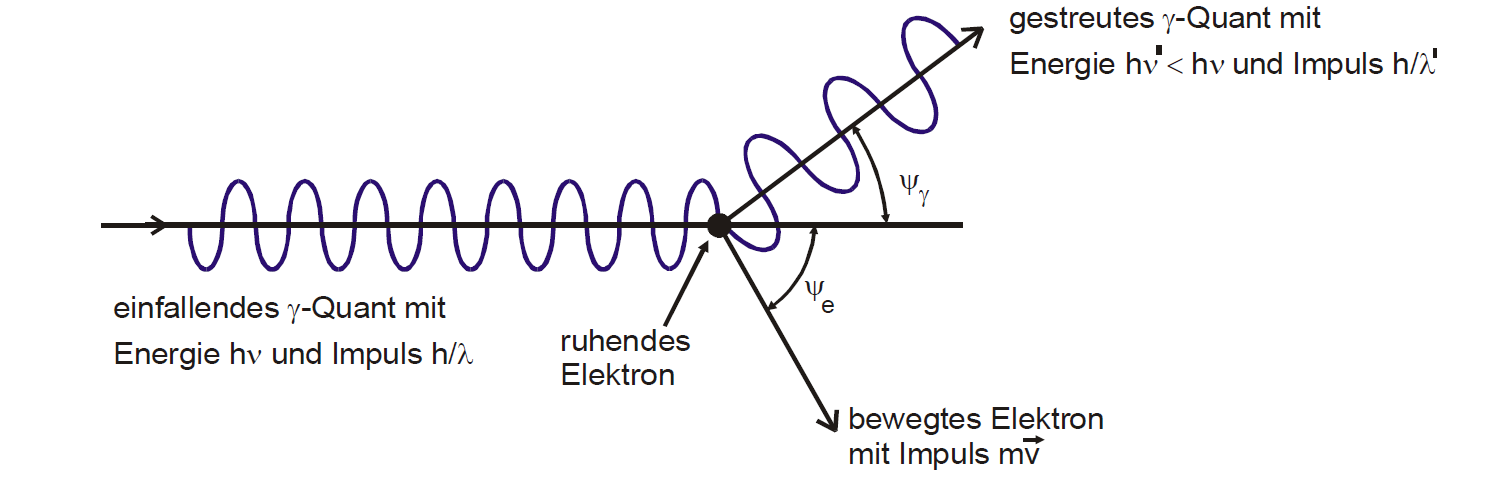
\includegraphics[width=0.9\textwidth]{ressources/compton.png}
  \caption{Vorgang beim Comptoneffekt, \cite{skript}.}
  \label{fig:compton}
\end{figure}
Ein Photon der Energie $E_\gamma$ stößt auf ein Elektron und gibt dabei einen Teil seiner Energie an das Elektron ab. Es handelt sich also um inelastische Streuung. Die Energie des gestreuten Elektrons ergibt sich hierbei zu
\begin{align}
  E_{e'} &= E_\gamma - E_{\gamma'} \\
  &= E_\gamma \frac{\varepsilon(1-\cos(\Psi_\gamma))}{1 + \varepsilon(1-\cos(\Psi_\gamma))} \; .
  \label{eq:comptonEnergie}
\end{align}
Hierbei bezeichnet $E_{e'}$ die Energie des gestreuten Elektrons, $E_{\gamma'}$ die Energie des gestreuten Photons, $\varepsilon=E_\gamma/m_e c^2$ und $\Psi_\gamma$ den Winkel des gestreuten Photons gegenüber einem ungestreuten Photon. Diese Energie wird maximal für $\Psi_\gamma = 180°$, also im Fall der Rückwärtsstreuung. Sie wird auch als Comptonkante bezeichnet, da oberhalb dieser Energie keine weitere Comptonstreuung stattfinden kann.
\begin{equation}
  E_{e',\text{max}} = E_\text{Comptonkante} = E_\gamma \frac{2\varepsilon}{1+2\varepsilon} < E_\gamma
  \label{eq:comptonEmax}
\end{equation}
 Hier nimmt der differentielle Wirkungsquerschnitt  ein Maximum an, siehe Abbildung \ref{fig:comptonWQ}. Es finden also überdurchschnittlich viele Compton-Streuprozesse unter Rückstreuung statt.
 \begin{figure}
   \centering
   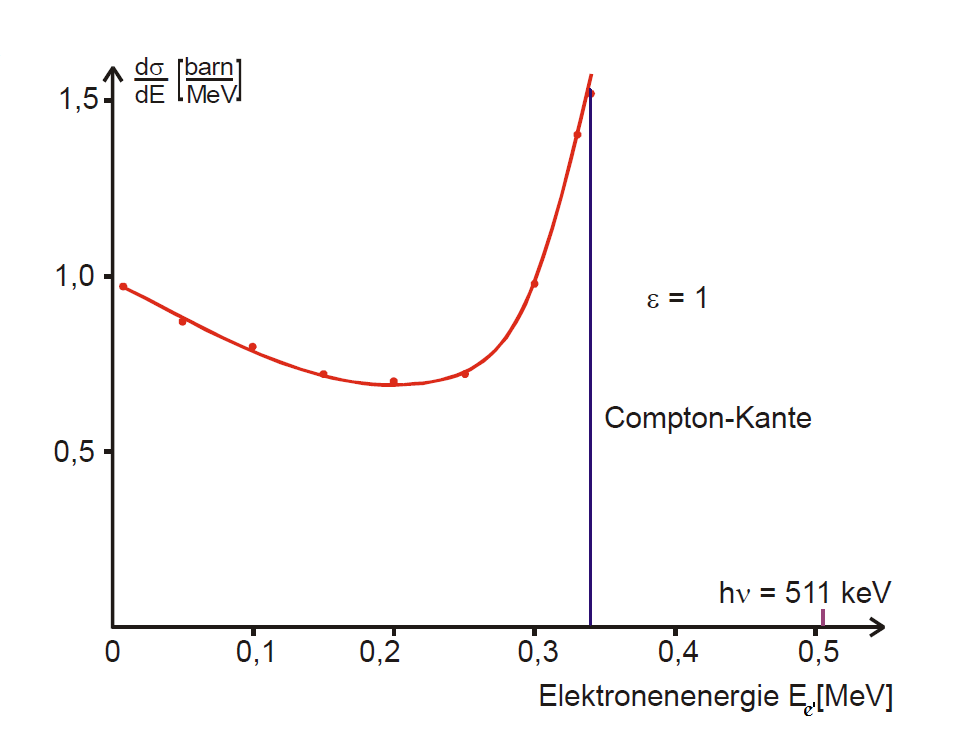
\includegraphics[width=0.7\textwidth]{ressources/compton2.png}
   \caption{Differentieller Wirkungsquerschnitt als Funktion der Energie des gestoßenen Elektrons $E_{e'}$ für $\varepsilon=1$. Eingezeichnet ist die Comptonkante, sowie weiter rechts die Ruheenergie des Elektrons von $\SI{511}{\kilo\electronvolt}$, nach \cite{skript}.}
   \label{fig:comptonWQ}
 \end{figure}
 Das Photon verliert in diesem Fall gerade die Energie $E_{e',\text{max}}$. Es kann dann erneut eine Compton-Streuung auslösen, siehe Kapitel \ref{sec:vorgaenge}.

 \subsubsection{Paarerzeugung}
Für diesen Effekt muss die Energie des Photons ausreichend groß sein, um unter Anwesenheit eines Stoßpartners in ein Elektron und ein Positron zu zerfallen. Der Stoßpartner nimmt dabei den Impuls des Photons auf. Infolge der stark unterschiedlichen Massen von Elektron und Atom macht es für die Schwellenenergie $E_\text{min}$ einen Unterschied, mit welchem Stoßpartner das Photon interagiert. Im Falle eines Elektrons ergibt sich $E\text{min}=4m_e c^2$, im Falle eines Atoms $E_\text{min}=2m_e c^2$. Die unterste Grenze für den Effekt der Paarerzeugung beträgt also ca. $\SI{1}{\mega\electronvolt}$. Allerdings ist dieser Vorgang unwahrscheinlich, da Elektron und Positron in diesem Fall keine kinetische Energie besitzen. Eine sinnvolle Richtgröße ist daher ein Wert von ca.
\begin{equation}
  E_\text{min}\approx\SI{2}{\mega\electronvolt} \; .
\end{equation}
Die entstandenen Teilchen können in Folge weiterer Wechselwirkungen ihre kinetische Energie verlieren und rekombinieren. Bei dieser Paarvernichtung entstehen dann 2 Photonen mit jeweils der Energie der Ruhemasse eines Elektrons, also $\SI{511}{\kilo\electronvolt}$.\\
Der Wirkungsquerschnitt hängt davon ab, wo die Paarerzeugung stattfindet. Während in kernnahen Schalen wie der k-Schale das Coulombfeld des Kerns kaum abgeschirmt ist, ist diese Abschirmung für einen Prozess außerhalb der Elektronenhülle vollständig. In letzterem Fall wird der Wirkungsquerschnitt energieunabhängig, während bei verschwindender Abschirmung der Wirkungsquerschnitt logarithmisch mit $\varepsilon$ geht. Beiden gemeinsam ist eine Proportionalität zu der Kernladungszahl $Z$.

\subsubsection{Zusammenfassung der Effekte}
In Abbildung \ref{fig:extinktionskoeffizient} ist der Extinktionskoeffizient aus Gleichung \eqref{eq:extinktion} für einen Energiebereich über vier Größenordnungen doppelt-logarithmisch aufgetragen. Er ergibt sich aus der Summe der zuvor beschriebenen Effekte.
\begin{figure}
  \centering
  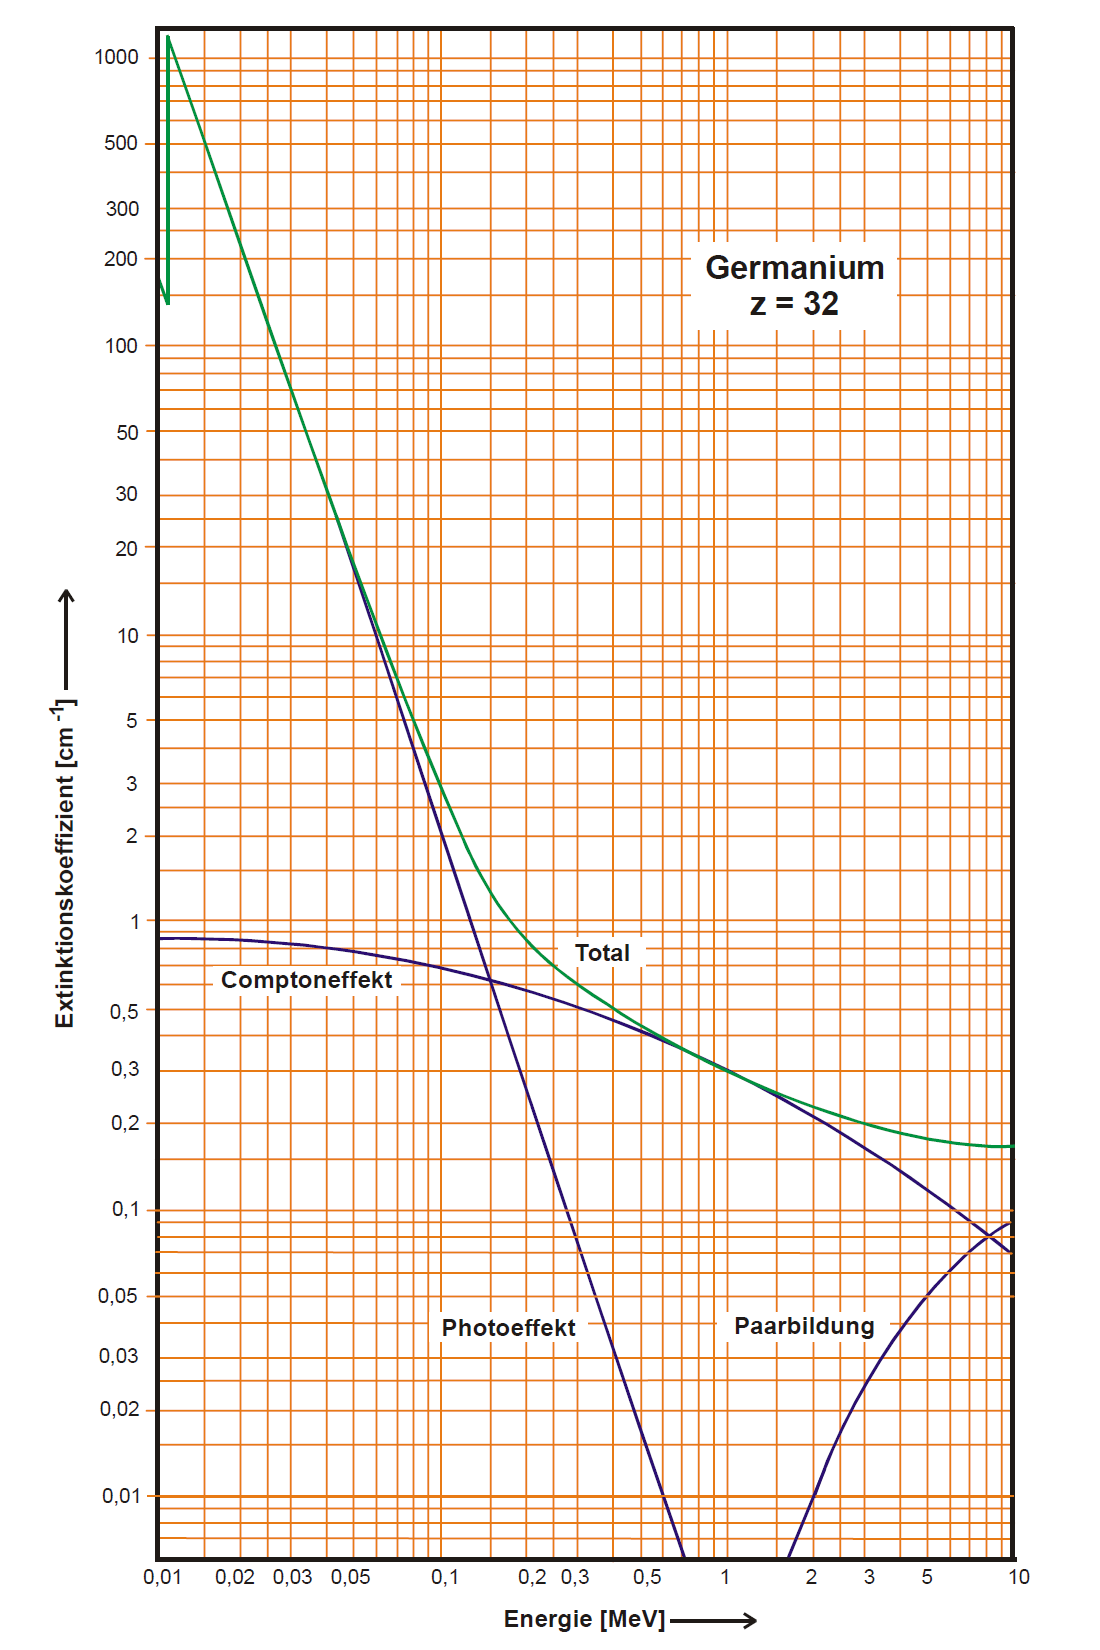
\includegraphics[width=0.8\textwidth]{ressources/extinktionskoeffizient.png}
  \caption{Extinktionskoeffizient in Abhängigkeit der Energie des einfallenden Photons, \cite{skript}.}
  \label{fig:extinktionskoeffizient}
\end{figure}
Zu erwähnen ist insbesondere der Schnittpunkt zwischen Compton- und Photoeffekt bei ca. $\SI{130}{\kilo\electronvolt}$. Für größere Energien ist die Wahrscheinlichkeit für das Eintreten eines Comptoneffektes gegenüber dem eines Photoeffektes zunehmend größer.


\subsection{Der Germaniumdetektor}
\label{sec:detektor}
Der Reinst-Germanium-Detektor ist ein Halbleiterdetektor. Einfallende Photonen werden innerhalb der Verarmungszone zwischen p- und n-dotiertem Bereich detektiert, indem die in Folge der in Kapitel \ref{sec:ww} beschriebenen Effekte entstehenden Ladungsträger abgesaugt werden und somit zu einem Ladungsimpuls beitragen. Dieser wird durch eine geeignete Elektronik ausgelesen.

\subsubsection{Der pn-Übergang}
\label{sec:pn}
Abbildung \ref{fig:pn} zeigt das Bänderdiagramm eines pn-Übergangs von Silizium, welches sich aber direkt auf den vorliegenden Germanium-Detektor übertragen lässt.
\begin{figure}
  \centering
  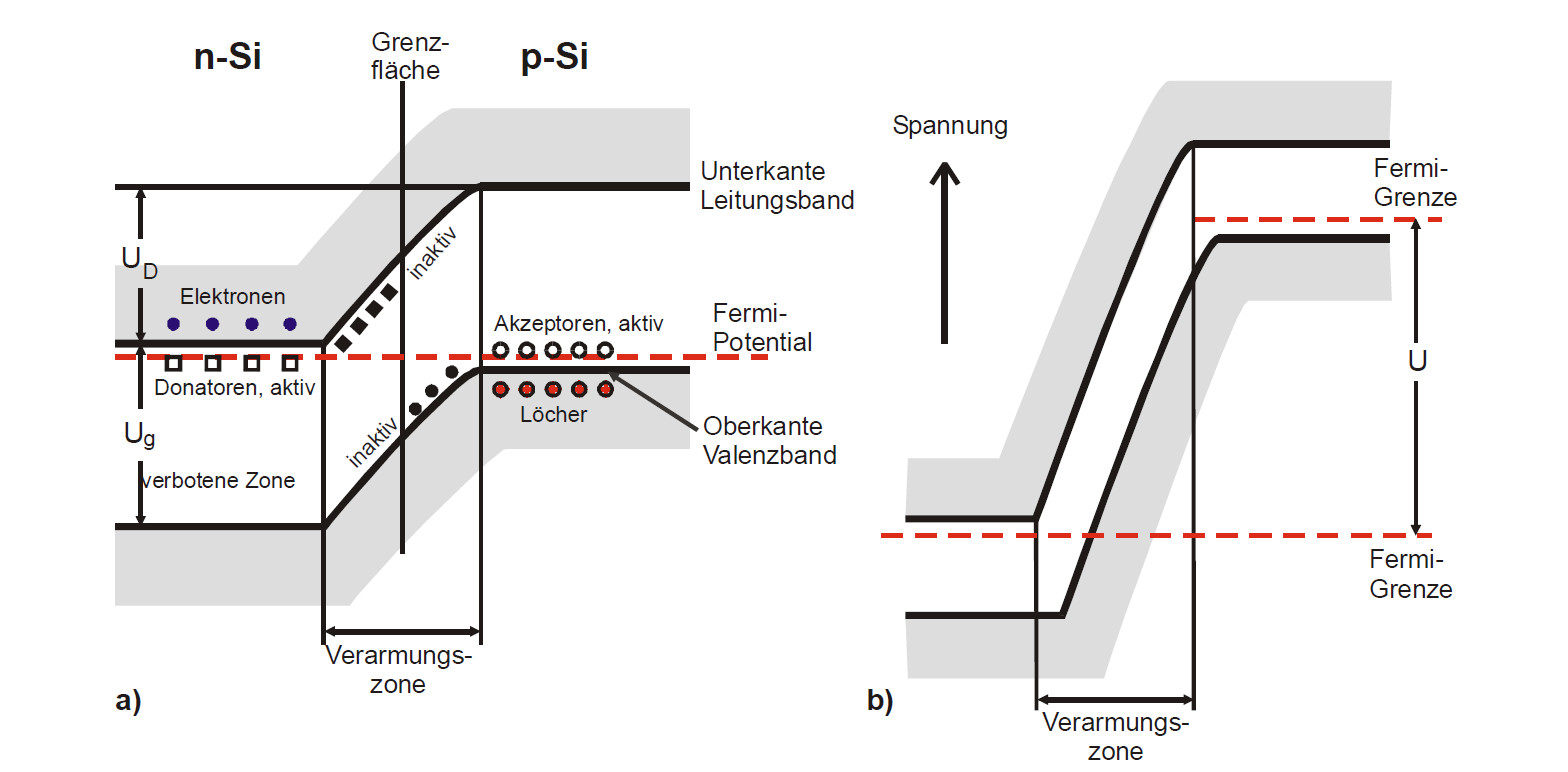
\includegraphics[width=0.9\textwidth]{ressources/pn.png}
  \caption{Bänderdiagramm beim pn-Übergang. a) intrinsisch ohne äußere Spannung, b) mit angelegter Spannung in Sperrrichtung, \cite{skript}.}
  \label{fig:pn}
\end{figure}
Ladungsträger diffundieren durch die Verarmungszone und rekombinieren dort. Die zurückbleibenden, lokalen Akzeptoren und Donatoren bilden daraufhin ein gegenläufiges elektrisches Feld aus, bis es zu einem Gleichgewicht kommt. Die so entstehende Potentialdifferenz zwischen den Leitungsbändern im n- und p-dotierten Bereich wird Diffusionsspannung $U_D$ bezeichnet. Sie bildet einen Potentialwall, siehe Abbildung \ref{fig:pn}a). Dieser kann durch Anlegen einer äußeren Spannung zwischen n- und d-Bereich weiter erhöht werden (Abbildung \ref{fig:pn}b)$\,$). Die externe Spannung wird als Sperrspannung $U$ bezeichnet. In der Verarmungszone liegt daher bei angelegter Sperrspannung ein elektrisches Feld vor, welches dazu in der Lage ist, Ladungsträger, die in der Zone entstehen nach ihrer Polarität zu trennen, bevor sie rekombinieren können. Diese Eigenschaft bildet die Grundlage des Detektors. \\
Um nun möglichst viele einfallende Photonen zu detektieren ist es gemäß Gleichung \eqref{eq:extinktion} günstig, die Tiefe der Verarmungszone zu maximieren. Diese liegt bei einer herkömmlichen Diode im Bereich von einigen $\si{\micro\meter}$ \cite{skript}, kann aber durch das Anlegen einer möglichst großen Sperrspannung sowie einer geeigneten Dotierung auf einige $\si{\centi\meter}$ vergrößert werden. Die Dotierung muss dabei so gewählt werden, dass eine Seite des Übergangs sehr stark, und die andere Seite sehr schwach dotiert ist. Im vorliegenden Germanium Detektor ist das Germanium mit $n_A\approx 10^{10}$ Atome/$\si{\cubic\centi\meter}$ ein sehr schwach p-dotierter Halbleiter und wird daher auch als \emph{Reinst-}Germanium bezeichnet. Die hohe n-Dotierung wird durch Eindiffusion von Li Atomen auf der Oberfläche erreicht, siehe Abbildung \ref{fig:aufbauDetektor}. Unter diesen Voraussetzungen lässt sich die Dicke der Verarmungszone zu
\begin{equation}
  d \approx \sqrt{\frac{2\epsilon_{r,\text{Ge}}\epsilon_0 ( U_D + U)}{n_A e}}
  \label{eq:dicke}
\end{equation}
abschätzen.\\
Die zweite Möglichkeit, die Breite der Verarmungszone zu maximieren, ist das Anlegen einer möglichst großen Sperrspannung. Diese ist jedoch nach oben hin limitiert aufgrund des Leckstroms. Ladungsträger können durch thermische Aktivierung in der Verarmungszone entstehen, wenn die thermische Energie größer oder gleich dem Abstand zwischen Leitungskante und Störstellenniveau ist. Im Bereich niedriger Temperaturen werden nicht alle durch Dotierung eingebrachten Ladungsträger angehoben, weshalb die Elektronenkonzentration im Leitungsband mit zunehmender Temperatur weiter zunimmt. Der Bereich wird als Störstellenreserve bezeichnet. Die Ladungsträger, welche ihren Weg zum Leitungsband gefunden haben, werden aufgrund der angelegten Sperrspannung genauso wie die aus den Wechselwirkungseffekten entstehenden Elektronen abgesaugt und bilden somit einen Strom. Um nun diesen störenden Rausch- oder Leckstrom zu limitieren, muss der Detektor gekühlt werden. Dies geschieht im Versuch mit Hilfe von flüssigem Stickstoff bei einer Temperatur von $\SI{77}{\kelvin}$, sodass eine Sperrspannung von ca. $\SI{5}{\kilo\volt}$ eingestellt werden kann.

\subsubsection{Vorgänge im Detektor}
\label{sec:vorgaenge}
Mit Hilfe der in Kapitel \ref{sec:ww} erläuterten Effekte lässt sich eine Erwartung an das resultierende Spektrum formulieren. Ein Photon, welches den Detektor betritt hat typischerweise eine Energie im Bereich von mehreren hundert $\si{\kilo\electronvolt}$. Für diese Energien ist gemäß Abbildung \ref{fig:extinktionskoeffizient} das Eintreten eines Comptoneffektes am wahrscheinlichsten, und zwar um ca. 2 Größenordnungen wahrscheinlicher als der Photoeffekt. Paarbildung hingegen kann nicht stattfinden, da $E_\gamma < 2m_e c^2$. Das Photon wird also einen Streuprozess auslösen und dabei einen Teil seiner Energie verlieren, siehe Gleichung \eqref{eq:comptonEnergie}. Es können nun weitere Comptonstreuungen folgen. Diese Kette kann von einem einzigen Photoeffekt beendet werden, sodass das ursprüngliche Photon seine gesamte Energie deponiert. Dieser Vorgang ist schematisch in Abbildung \ref{fig:vorgaenge1} dargestellt. Andererseits kann das Photon ebenfalls nach ein oder mehreren Comptonstreuungen den Detektor verlassen und somit nicht seine gesamte Energie deponieren, siehe Abbildung \ref{fig:vorgaenge2}. \\
\begin{figure*}
    \centering
    \begin{subfigure}[b]{0.475\textwidth}
        \centering
        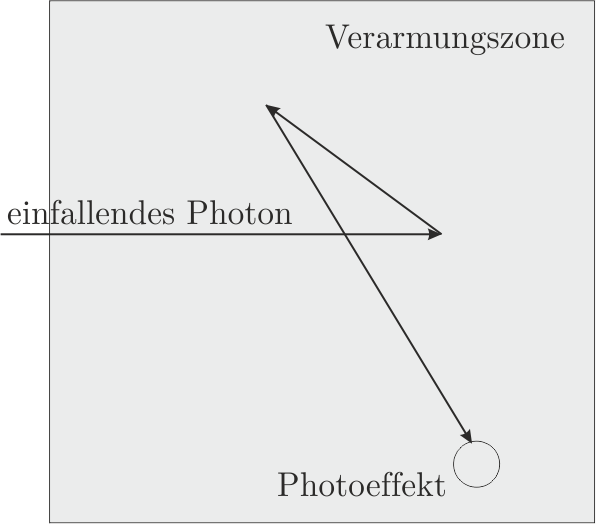
\includegraphics[width=\textwidth]{ressources/vorgaenge2.png}
        \caption[]%
        {{\small Die Kette von Comptonstreuungen wird durch einen einzigen Photoeffekt beendet.}}
        \label{fig:vorgaenge1}
    \end{subfigure}
    \hfill
    \begin{subfigure}[b]{0.475\textwidth}
        \centering
        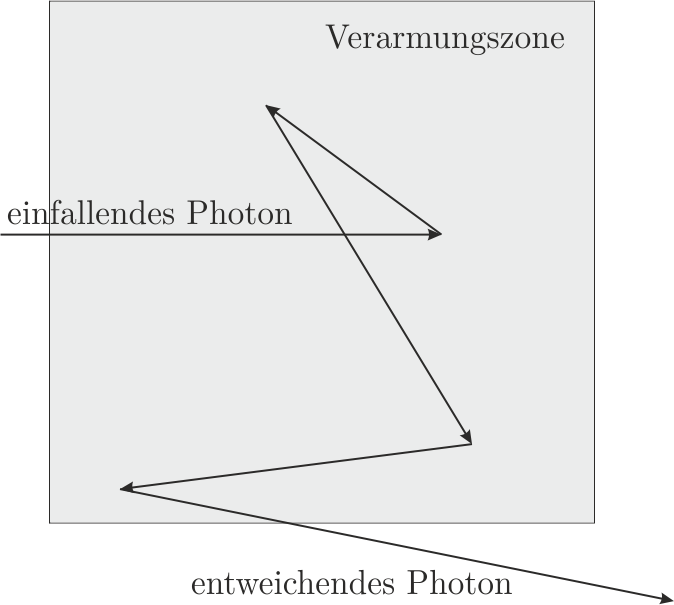
\includegraphics[width=\textwidth]{ressources/vorgaenge1.png}
        \caption[]%
        {{\small Ohne den Photoeffekt deponiert das Photon nicht seine gesamte Energie.}}
        \label{fig:vorgaenge2}
    \end{subfigure}
    \caption[]
    {Zwei mögliche Abläufe innerhalb der Verarmungszone.}
    \label{fig:vorgaenge}
\end{figure*}
Im ersten Fall entsteht ein sogenannter Vollenergiepeak. Die Menge der Elektronen, die bei dem gesamten Prozess (also ein oder mehrere Comptonstreuungen plus Photoeffekt) entstehen, wird dabei in sehr schneller zeitlicher Abfolge generiert, da das Photon mit Lichtgeschwindigkeit fliegt. Die Zeit hingegen, welche die Elektronen für ihren Weg zur Anode benötigen ist größer. Hinzu kommt, dass die Auswerteelektronik diese Ladungen über einen gewissen Zeitraum integriert (siehe Gleichung \eqref{eq:vvspannung}). Folglich wird die gesamte Energie des Photons als ein einziges Signal detektiert. Diese Energie ist dann gegenüber den mehr oder weniger zufällig verteilten Energien der durch Comptonstreuung erzeugten Ladungsträger ausgezeichnet. Es kommt mit zunehmender Messzeit zu dem eingangs erwähnten Vollenergiepeak. \\
Wie bereits erwähnt, werden im zweiten Fall (ein oder mehrere Comptonstreuungen), die Energien einigermaßen zufällig verteilt sein. Das liegt daran, dass der Wirkungsquerschnitt der Comptonstreuung nicht besonders stark variiert. Allerdings nimmt er doch für einen Winkel von $\Psi_\gamma = 180°$ ein Maximum an, siehe erneut Abbildung \ref{fig:comptonWQ}. Daher ist an der Comptonkante ein schwaches Maximum in dem ansonsten flachen Comptonkontinuum zu erwarten. Nun können auf diese Weise rückgestreute Photonen wie bereits in Kapitel \ref{sec:compton} beschrieben mit der Energie $E_{\gamma'} = E_\gamma - E_{e',\text{max}}$ erneut gestreut werden. Auch diese Streuung geschieht bevorzugt unter einem Winkel von 180°. Aus dieser Überlegung ergibt sich, dass nicht nur an der Comptonkante $E_{e',\text{max}}$, sondern auch links davon bei
\begin{equation}
  E_\text{Rückstreu} = \frac{2(E_\gamma - E_{e',\text{max}}) }{1+2\varepsilon(E_\gamma - E_{e',\text{max}})}
  \label{Ruckstreu_wichtig}
\end{equation}
ein Maximum zu erwarten ist, der sogenannte Rückstreupeak. Hierbei meint $\varepsilon(x) = x/m_e c^2$.\\
Für kleiner werdende Photonenenergien wird in zunehmendem Maße Absorption außerhalb des Detektors an der Aluminium Schutzschicht des Detektors sowie auf der n-dotierten Oberfläche des Detektors bemerkbar. Unterhalb von ca. $\SI{40}{\kilo\electronvolt}$  können daher Photonen nicht mehr nachgewiesen werden. Dennoch wird das Comptonkontinuum nicht abrupt bei $\SI{40}{\kilo\electronvolt}$ beginnen, sondern vergleichsweise stetig von $E=0$ an ansteigen bis dorthin. Der Grund dafür liegt in den Photonen, die anfangs ausreichend Energie haben, den Detektor zu betreten (z.B. $\SI{60}{\kilo\electronvolt}$). Im Detektor werden sie dann gestreut und liefern z.B. einen Beitrag für $\SI{50}{\kilo\electronvolt}$. Auch die verbleibenden $\SI{10}{\kilo\electronvolt}$ können nun detektiert werden.\\
Für einen Monochromator, welcher einzig Photonen der Energie $E_0$ aussendet, wird gemäß den vorangegangenen Ausführungen ein einzelner Vollenergiepeak bei $E_0$ erwartet, während ein für die $\gamma$-Spektroskopie störendes Comptonkontinuum mit zwei schwachen Maxima überlagert ist.


\subsubsection{Auflösungsvermögen}
Das Auflösungsvermögen $\Delta E_{1/2}$ ist die wichtigste Kenngröße eines Detektors in der Spektroskopie. Es besagt prinzipiell, bis zu welchem energetischen Abstand zwei Peaks noch voneinander getrennt werden können. Die genaue Definition ist in Abbildung \ref{fig:aufl} dargestellt.
\begin{figure}
  \centering
  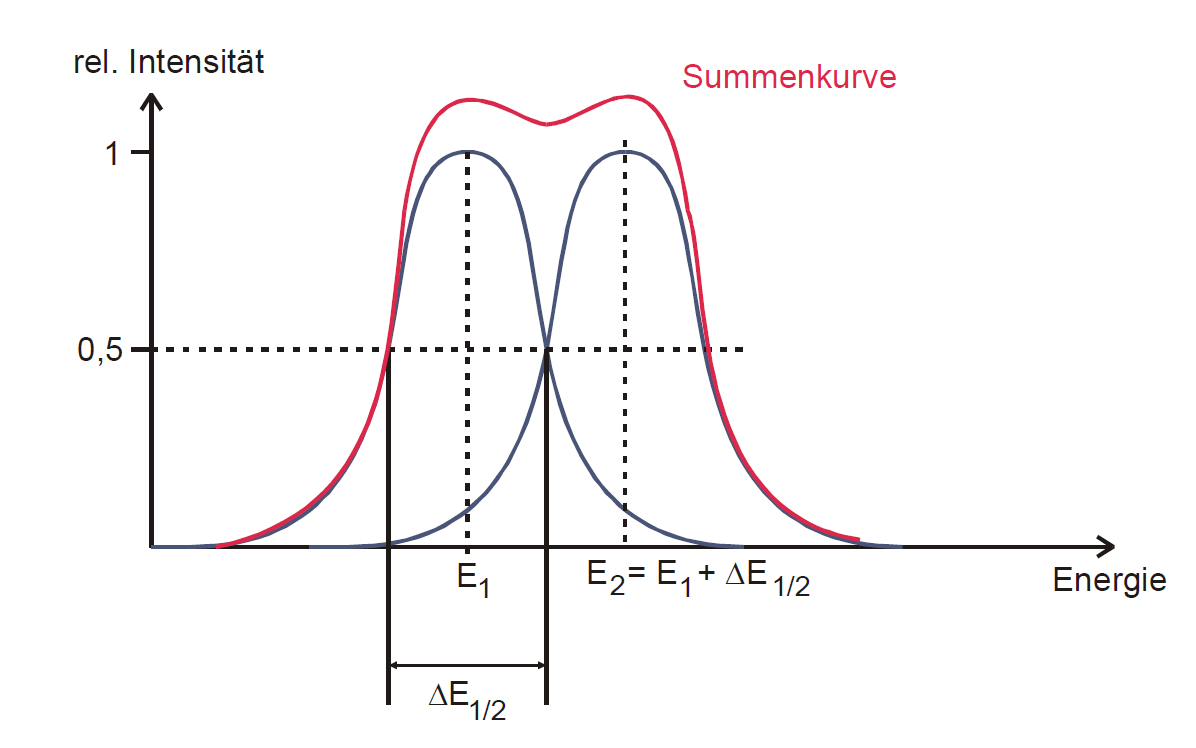
\includegraphics[width=0.7\textwidth]{ressources/aufl.png}
  \caption{Definition des Auflösungsvermögens $\Delta E_{1/2}$, \cite{skript}.}
  \label{fig:aufl}
\end{figure}
Zwei nebeneinander liegende Peaks, die sich auf der Hälfte ihrer Höhe schneiden haben per Definition den Abstand $\Delta E_{1/2}$. Ist dieser Wert klein, so sind entsprechend die Peaks scharf. Die Breite eines Peaks ergibt sich maßgeblich aus der Streuung der Anzahl $n$ der bei der Absorption eines Photons emittierten Elektron-Loch-Paare. Für diese Messgröße wird eine Poisson-Verteilung angesetzt. Da nun aber gleichzeitig bei der Entstehung von Elektron-Loch-Paaren auch Phononen beteiligt sind, muss auch deren Fluktuation bezüglich ihrer Anregung berücksichtigt werden. Sie kompensiert die Standardabweichung von $n$ maßgeblich, was durch den sogenannten Fano-Faktor $F$ beschrieben wird.
\begin{equation}
  \sigma = \sqrt{F\bar{n}} = \sqrt{F\frac{E_\gamma}{E_{EL}}}
  \label{eq:fano_halbwertsbreite}
\end{equation}
Für Germanium beträgt $F\approx0,1$ \cite{skript}. In obiger Gleichung beschreibt $E_{EL}$ die Energie zur Bildung eines Elektron-Loch-Paares. Sie setzt sich wesentlich aus der Energie der Bandlücke des Halbleiters zusammen. Aufgrund der Beteiligung der Phononen wird jedoch für Germanium ein Wert von $\SI{2,9}{\electronvolt} \approx 4E_g$ gemessen \cite{skript}.\\
Da $n$ groß ist, geht die Poissonverteilung in eine Gaußverteilung über. Es gilt
\begin{equation}
  \Delta E_{1/2} = \sqrt{8\text{ln}2} \frac{\sigma}{\bar{n}}E_\gamma \approx 2,35 \sqrt{0,1 E_\gamma E_{EL}}
  \label{eq:deltae}
\end{equation}
Allerdings beschreibt diese Gleichung lediglich eine Abschätzung, da zusätzlich weitere Störeinflüsse durch die elektrische Schaltung oder auch die in Kapitel \ref{sec:pn} beschriebene thermische Anregung hinzukommen. Dennoch ist ersichtlich, dass der Fano-Faktor sowie die Energie der Elektron-Loch-Paar Erzeugung eine wichtige Rolle spielen. Für Germanium stellt sich ein vergleichsweise kleiner Fano-Faktor ein. Außerdem ist auch $E_{EL}$ klein aufgrund der kleinen Bandlücke von Germanium $E_g = \SI{0,661}{\electronvolt}$ bei $T=\SI{300}{\kelvin}$ \cite{Egap}. Es ergibt sich bei einer Energie $E_\gamma = \SI{500}{\kilo\electronvolt}$ ein Auflösungsvermögen von $\SI{895}{\electronvolt}$.

\subsubsection{Effizienz}
\label{sec:effizienz}
Die Effizienz beschreibt die Nachweiswahrscheinlichkeit für ein einfallendes Photon. Bei der $\gamma$-Spektroskopie werden lediglich Prozesse betrachtet, die in einem Photoeffekt enden. Das heißt nach den Ausführungen aus Kapitel \ref{sec:photo} und Kapitel \ref{sec:vorgaenge}, dass die gesamte Energie des Photons umgesetzt und detektiert wird. Betrachtet werden also lediglich die Vollenergiepeaks. Unter Kenntnis der energieabhängigen Effizienz des Detektors lässt sich durch Messung auf die Aktivität $A(E)$ eines Strahlers rückschließen.
\begin{equation}
  A(E) = \frac{4\pi Z(E)}{\Omega W(E) Q(E)}
  \label{eq:effizienz}
\end{equation}
Hierbei beschreibt $\Omega$ den Raumwinkel, welchen der Detektor aus Sicht der Strahlungsquelle abdeckt, $W(E)$ die Emissionswahrscheinlichkeit eines Photons der Energie $E$ und $Z(E)$ die Zählrate. Die Emissionswahrscheinlichkeiten sind tabelliert. Der Raumwinkel ergibt sich aus der Anordnung des Versuchs, siehe Gleichung \eqref{eq:raumwinkel}. Die Zählrate ergibt sich aus dem Messwert der Auswerteelektronik des Detektors für den jeweiligen Vollenergiepeak der Energie $E$ (Counts innerhalb des Peaks) geteilt durch die Aktivzeit der Messung.
